\subsubsection{Stony Brook University}  
A TPC prototype has been constructed and a sophisticated test-beam setup established. We purchased picoammeter from PicoLogic in Zagreb/Croatia which is a unique device that allows to measure very small currents at high potential. The floating current measurements can be performed at potentials much larger than 5 kV, ideally suited for IBF measurements in a TPC.

The TPC prototype has been equipped with a real size readout module, based on a quadruple-GEM stack similar to the ALICE-TPC readout and zig-zag pad readout structure. The prototype has been exposed to the 120 GeV protons at the Fermilab Testbeam Facility (FTBF) to establish the working parameters of the TPC. We have analyzed the data obtained from the test-beam campaign and verified the performance parameter of the prototype.

We have continued to install components of the electron-/ion-gun for the evaporation of thin layer structures on mirror surfaces. The installation is running smoothly and undergraduate students are gaining experience in handling the sensitive equipment under the supervision of senior personnel. The installation process also helps in understanding the equipment and in preparing the start-up procedure of operation.

\begin{figure}
    \centering
    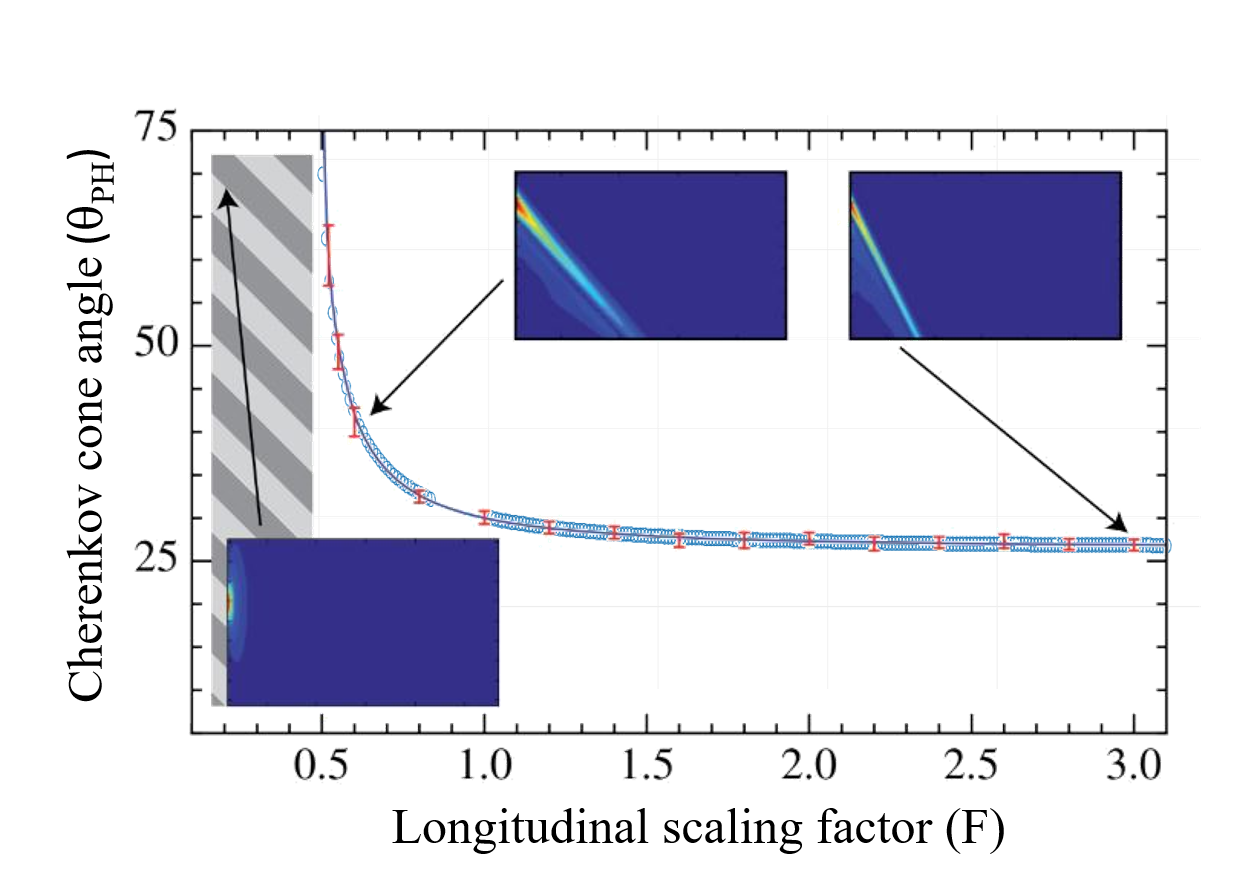
\includegraphics[width=0.8\columnwidth]{SBU_plots/phiVsFoverlayed.png}
    \caption{Reproduction of data based on the calculations obtained from the transformation metrics.}
    \label{fig:phiVsF}
\end{figure}
\begin{figure}
    \centering
    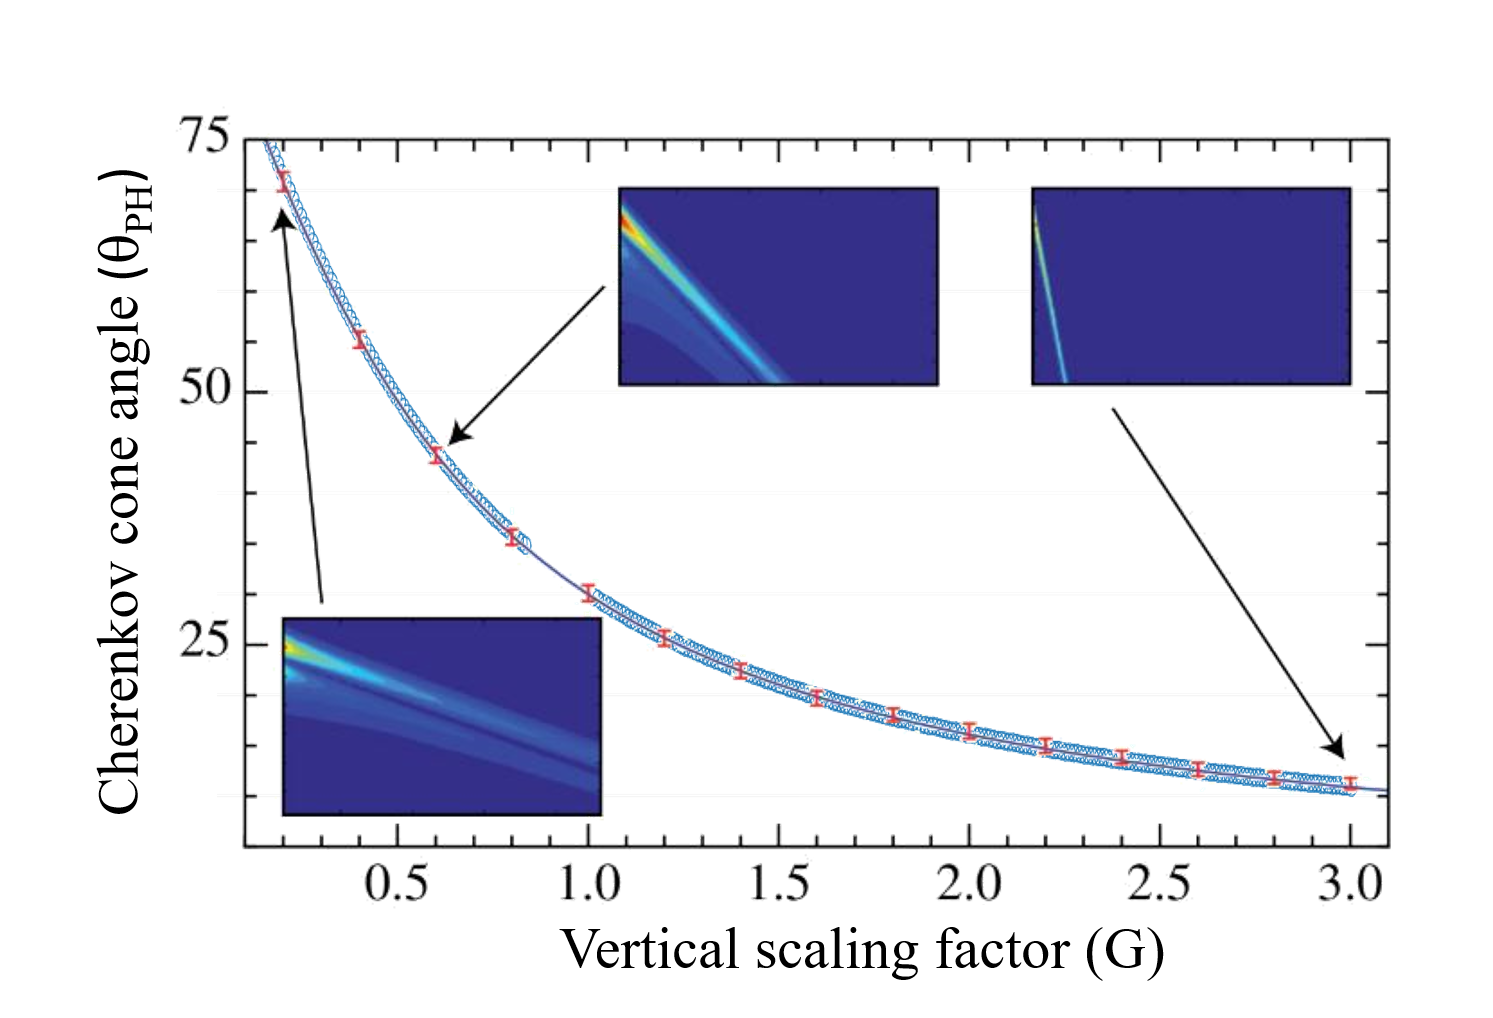
\includegraphics[width=0.8\columnwidth]{SBU_plots/phiVsGoverlayed.png}
    \caption{Reproduction of data based on the calculations obtained from the transformation metrics.}
    \label{fig:phiVsG}
\end{figure}